\chapter{DSD - Design Sequence Diagram}

\section*{1. addKitchenShift(shift, date, time, location?)}

\begin{center}
  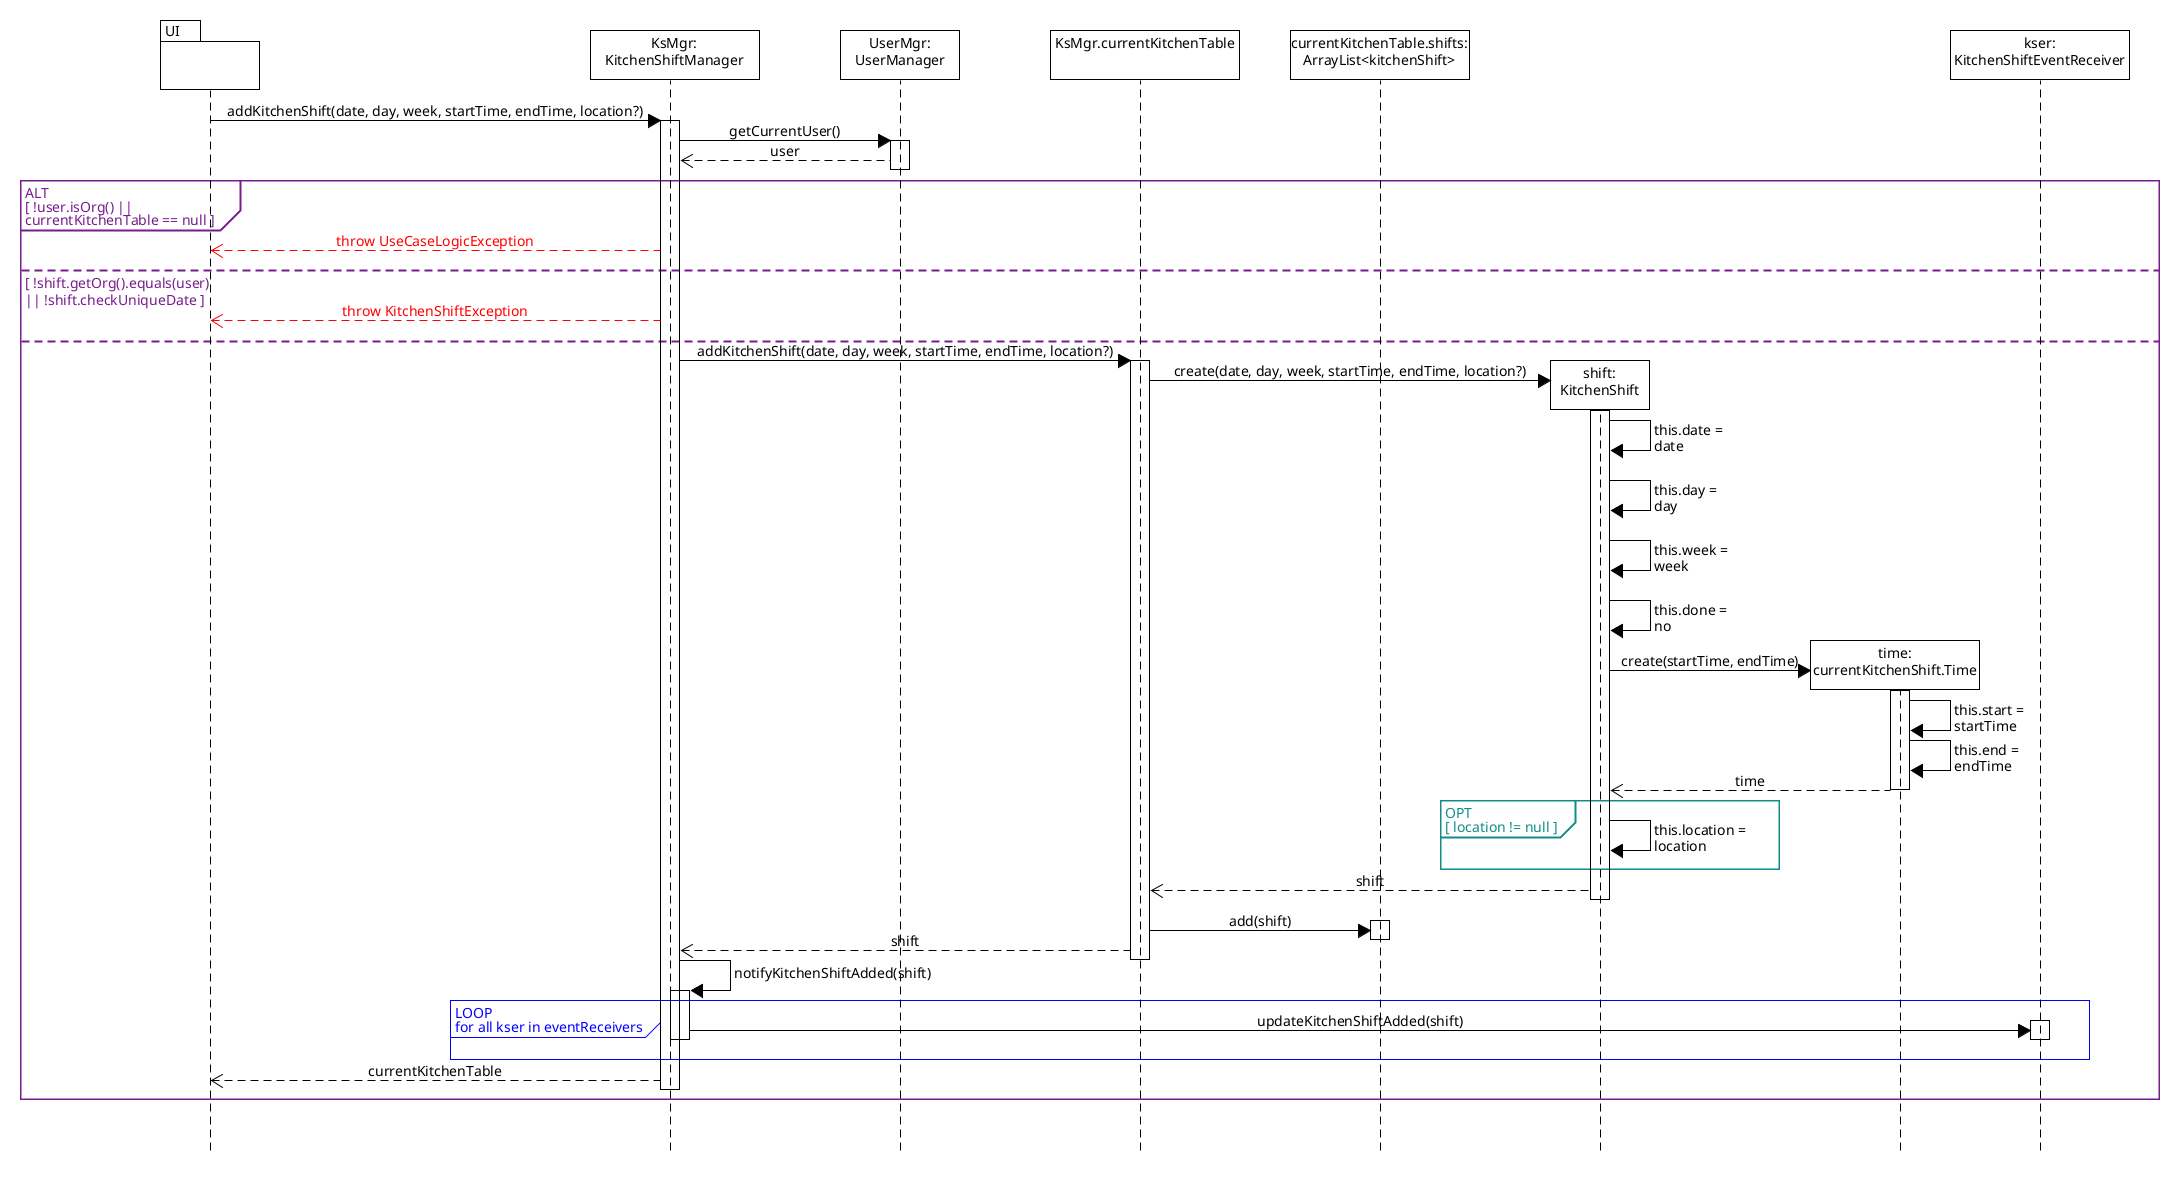
\includegraphics[scale = 0.2]{images/DSD/Esame DSD 1.png}
\end{center}

\begin{center}
  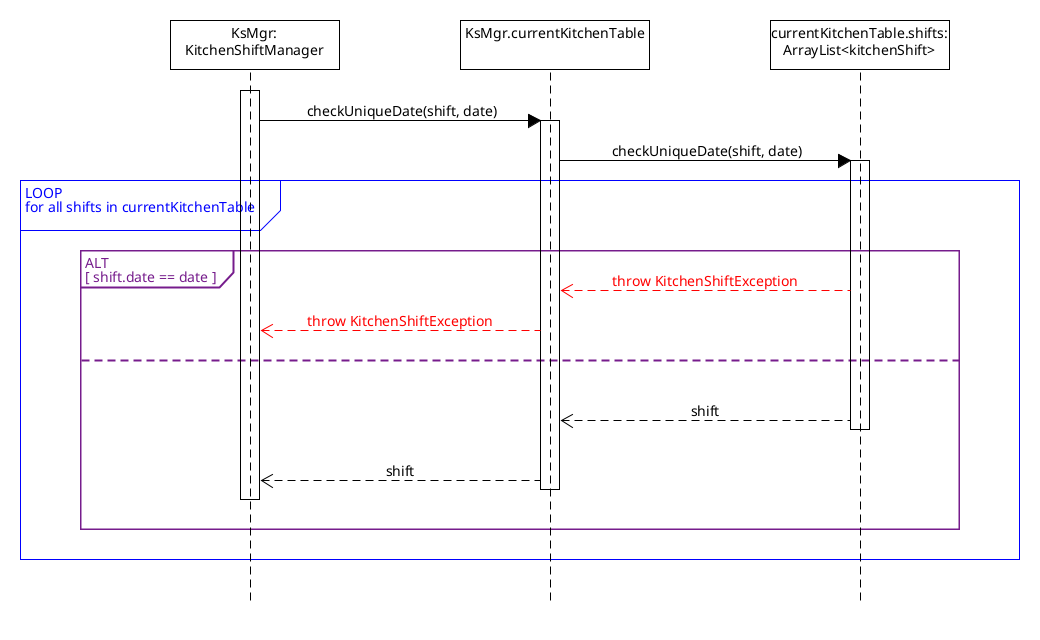
\includegraphics[scale = 0.4]{images/DSD/Esame DSD 1 Extra.png}  
\end{center}

\pagebreak

\section*{1c. editAllShifts(date, time?, location?)}

\begin{center}
  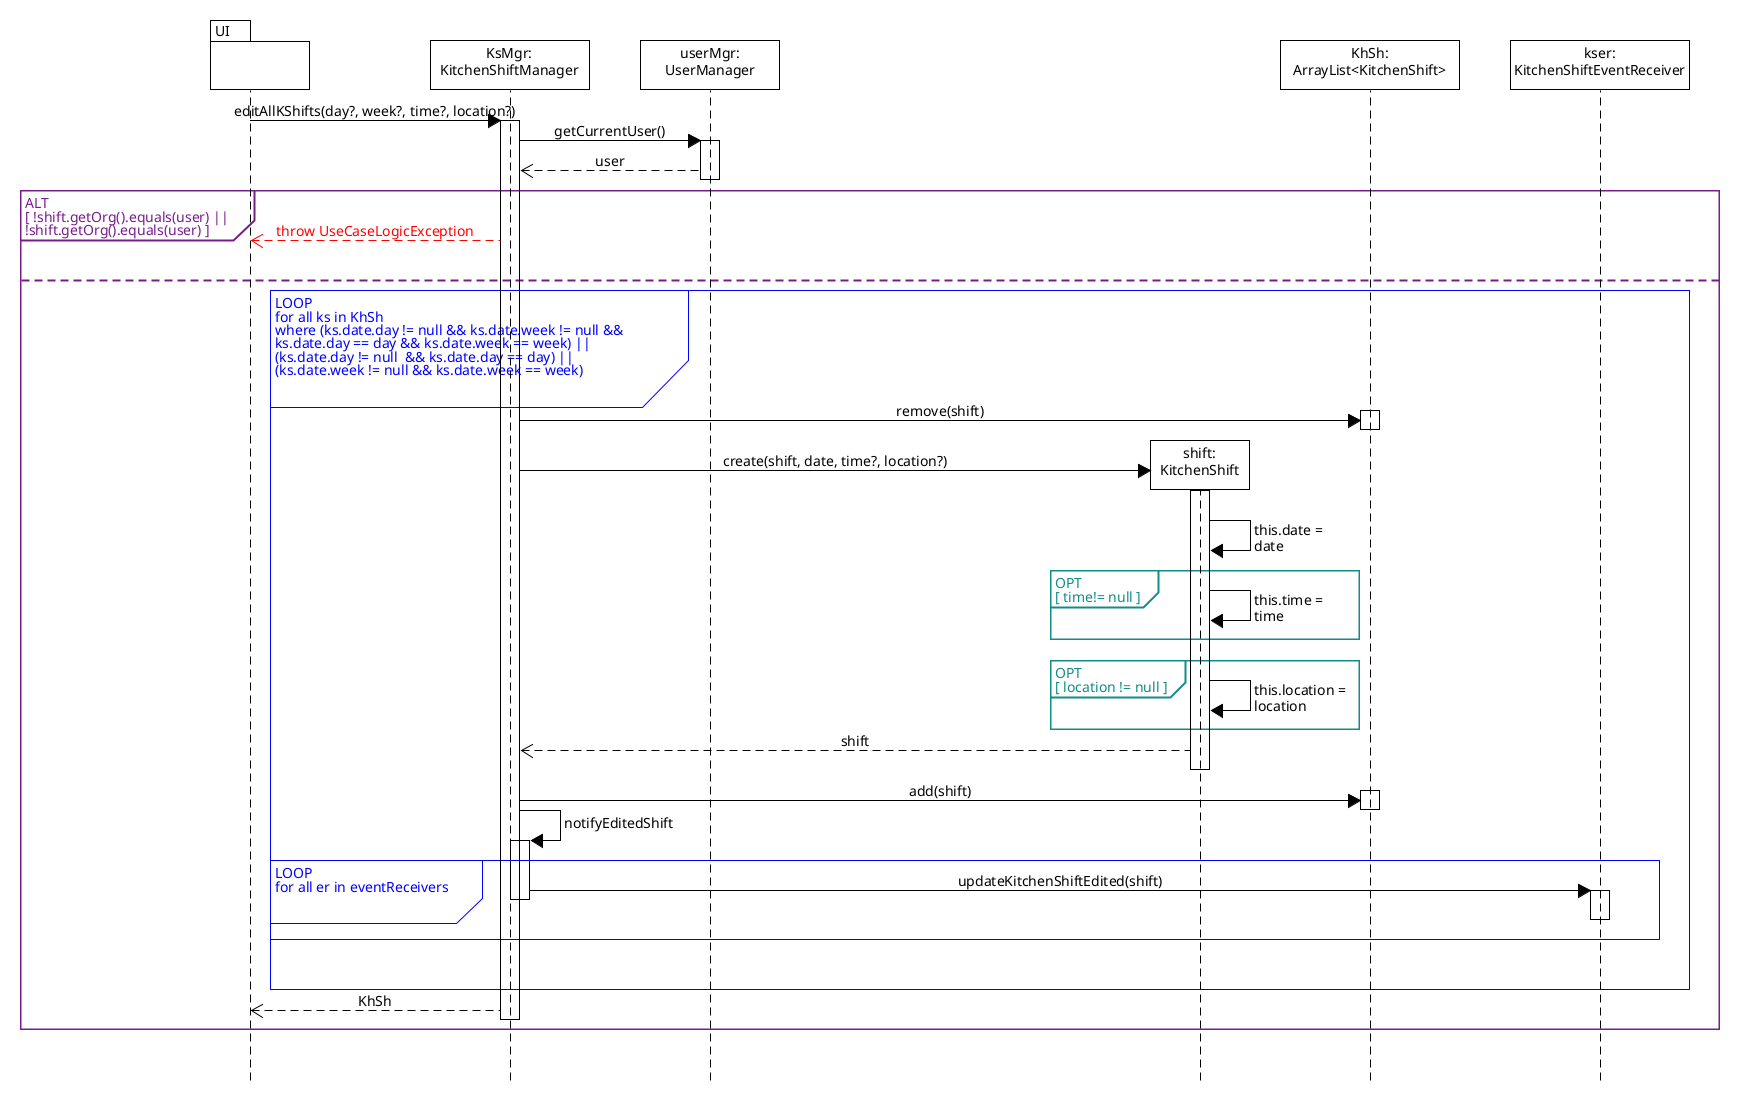
\includegraphics[scale = 0.28]{images/DSD/Esame DSD 1c.png}
\end{center}
\pagebreak
\section*{5. addTerm(serviceShift, term)}

\begin{center}
  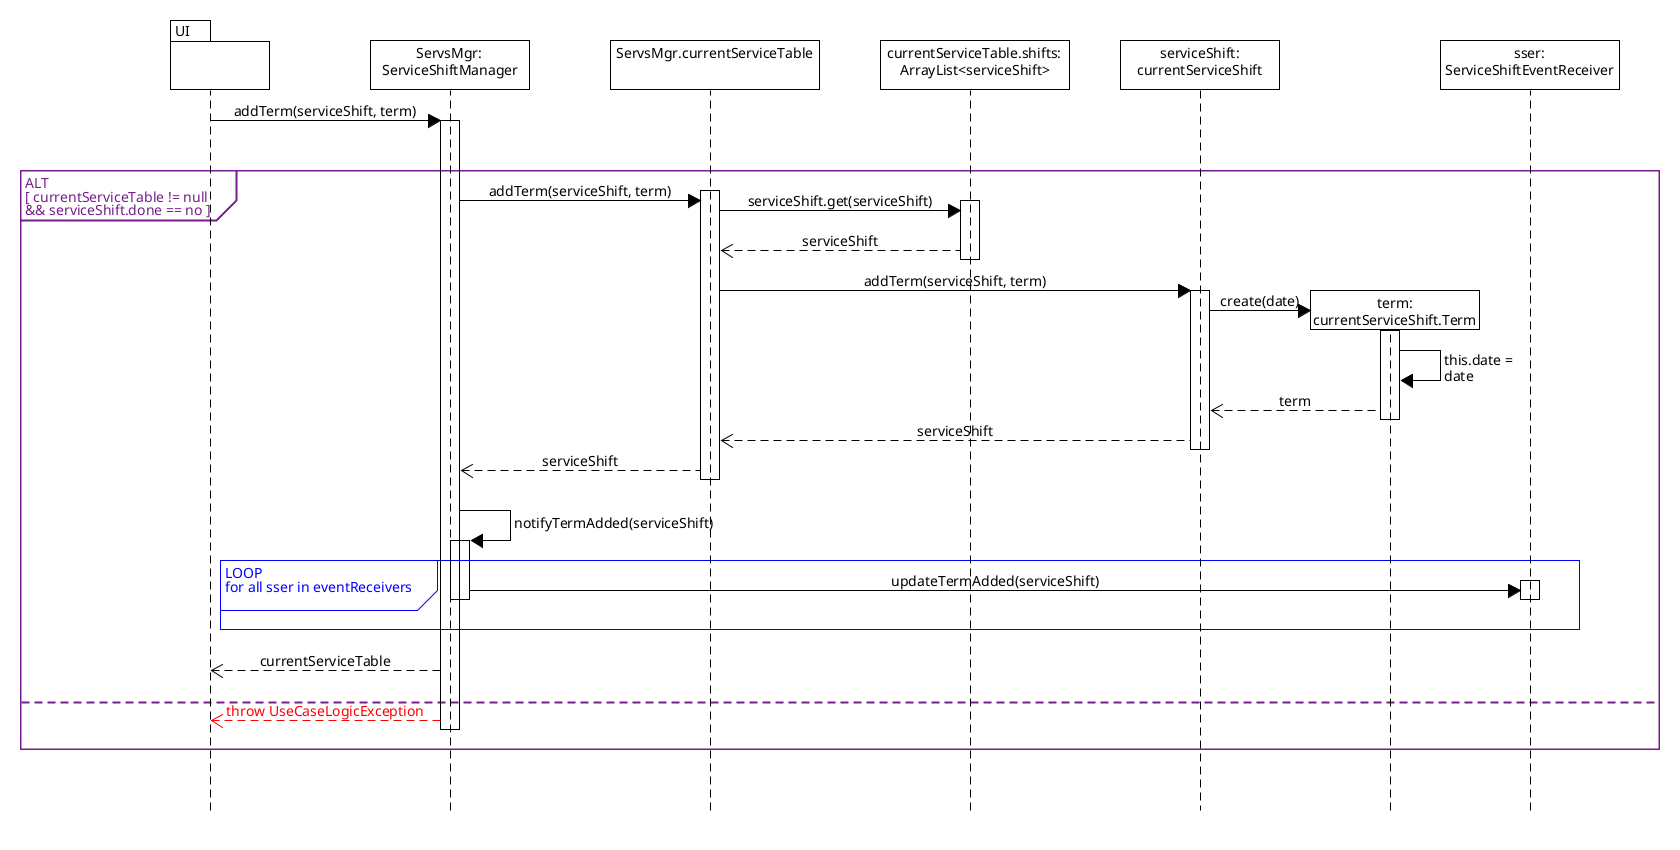
\includegraphics[scale = 0.28]{images/DSD/Esame DSD 5.png}
\end{center}
\pagebreak
\section*{6. editTime(serviceShift, newTime)}

\begin{center}
  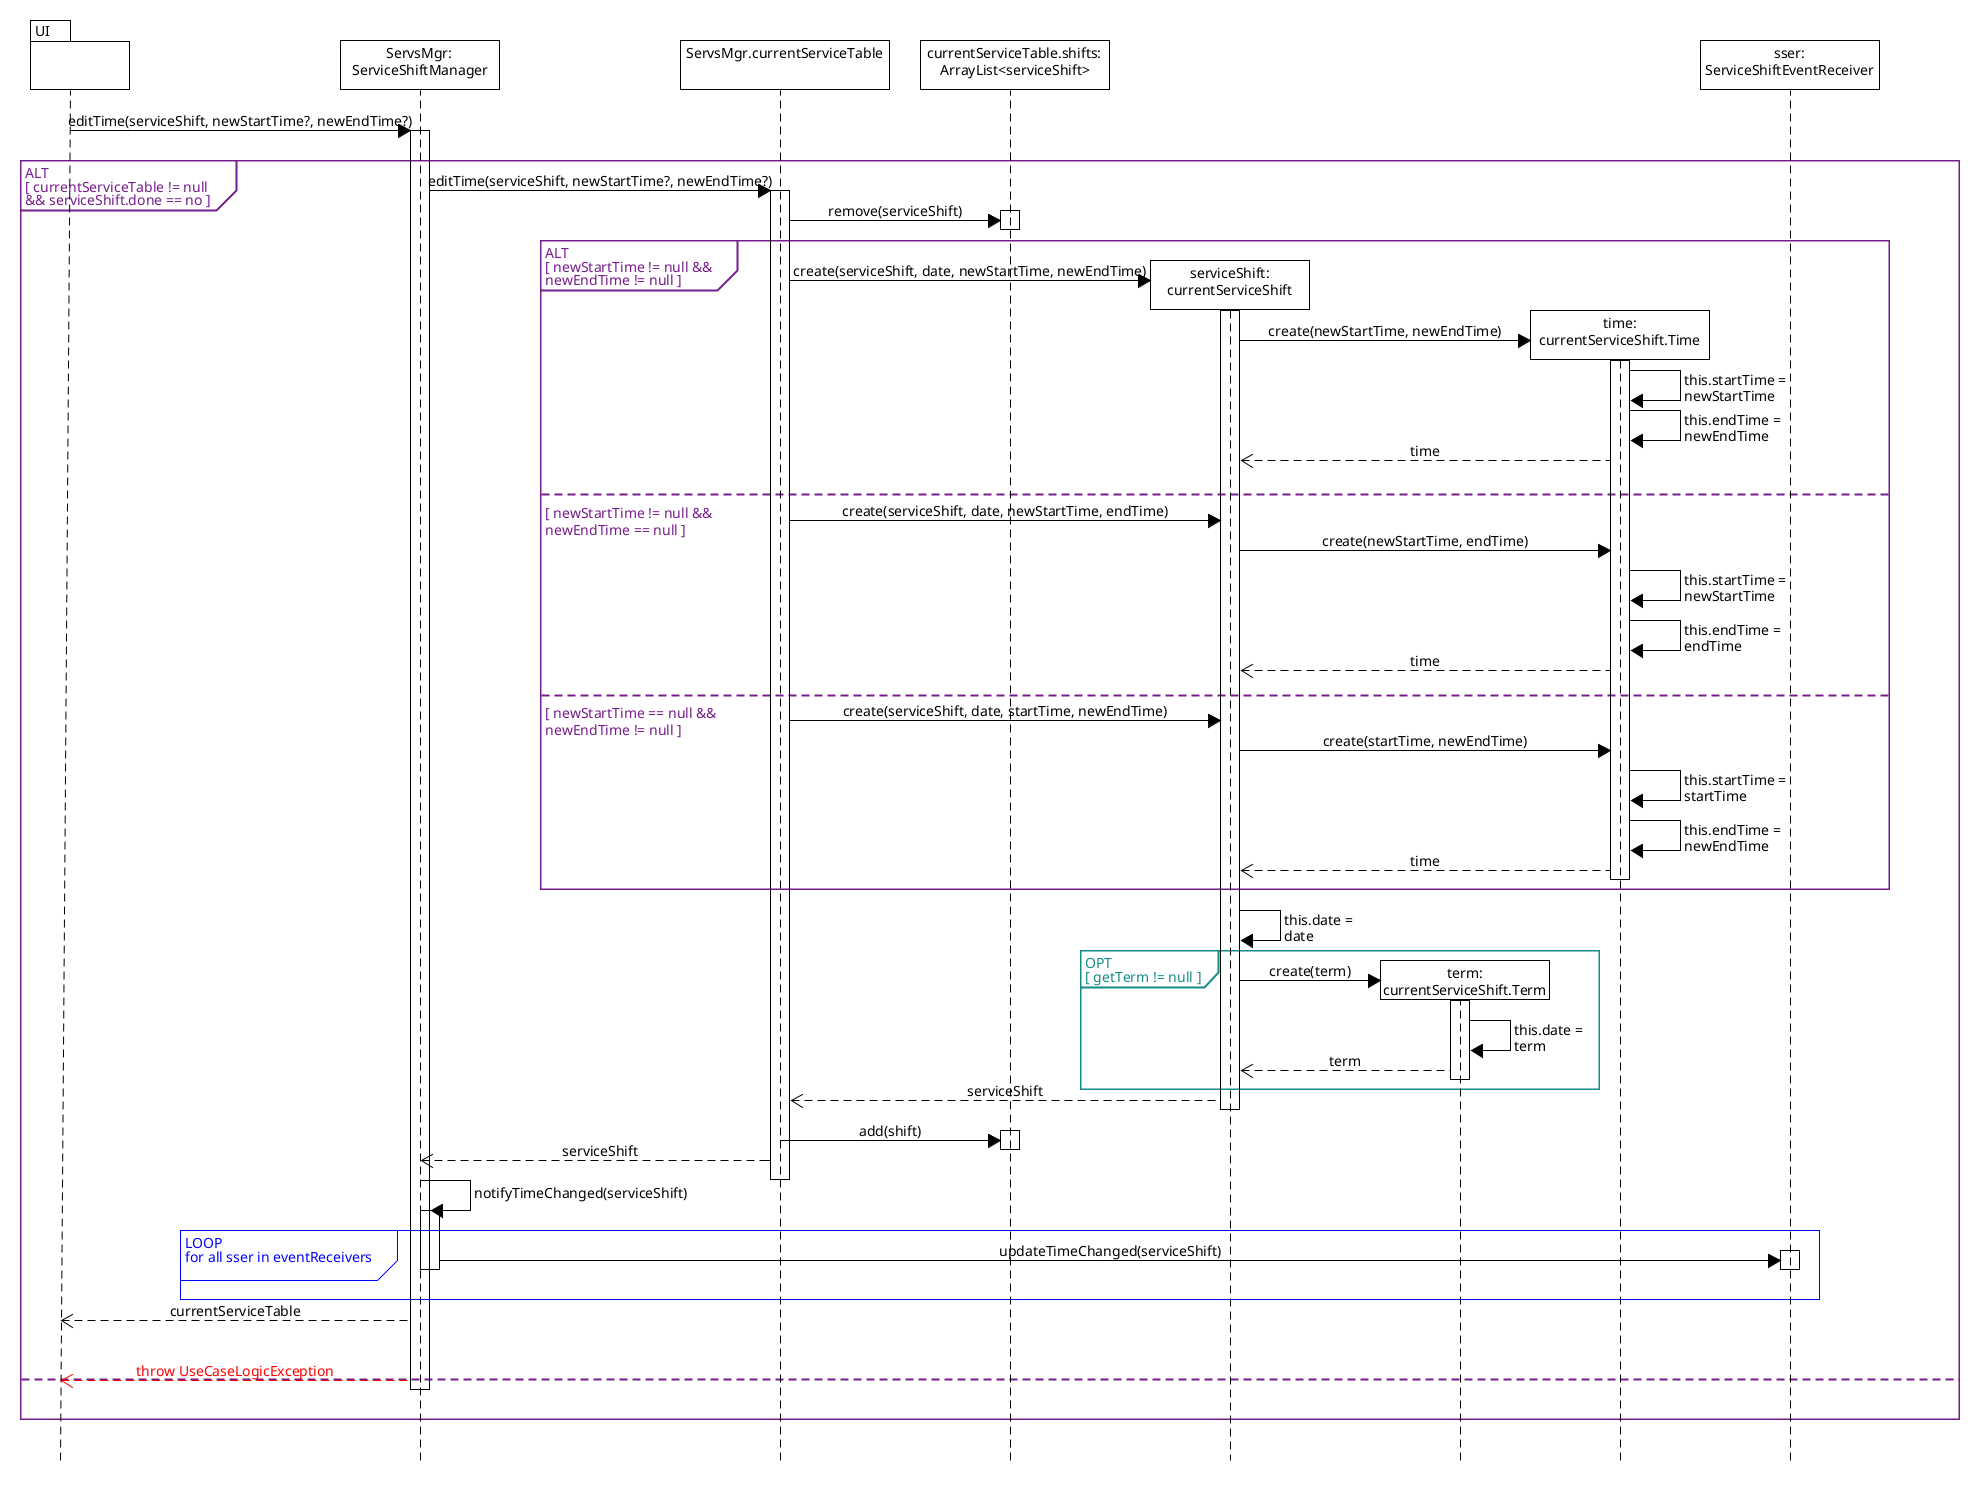
\includegraphics[scale = 0.24]{images/DSD/Esame DSD 6.png}
\end{center}
\pagebreak

\section*{6a. deleteServiceShift(serviceShift)}

\begin{center}
  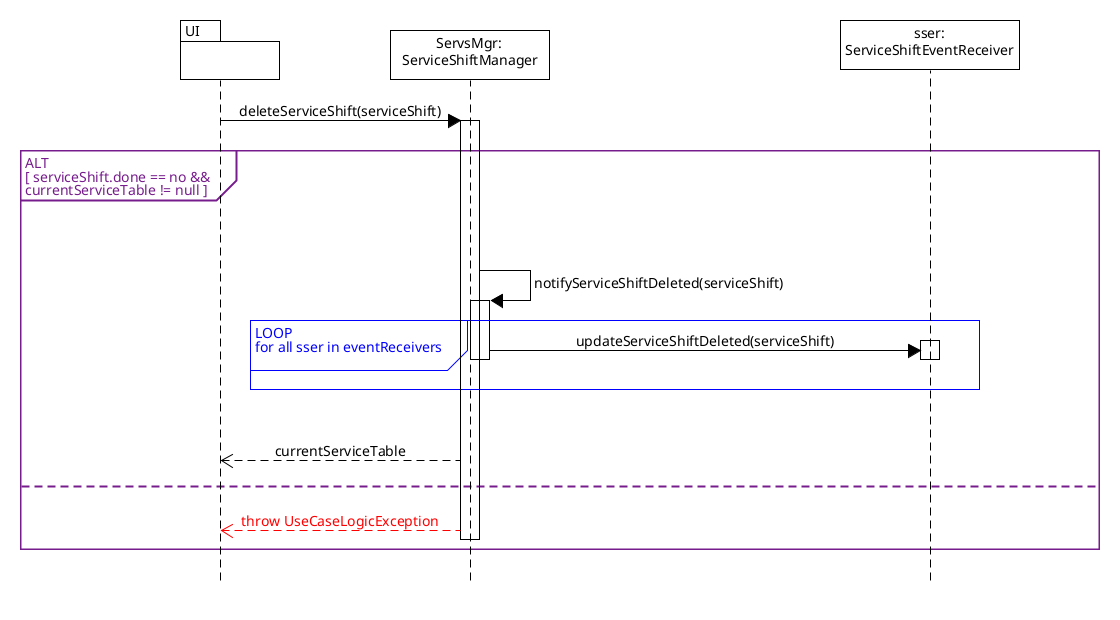
\includegraphics[scale = 0.28]{images/DSD/Esame DSD 6a.png}
\end{center}
\pagebreak
